% Options for packages loaded elsewhere
\PassOptionsToPackage{unicode}{hyperref}
\PassOptionsToPackage{hyphens}{url}
\PassOptionsToPackage{dvipsnames,svgnames,x11names}{xcolor}
%
\documentclass[
  letterpaper,
  DIV=11,
  numbers=noendperiod]{scrartcl}

\usepackage{amsmath,amssymb}
\usepackage{iftex}
\ifPDFTeX
  \usepackage[T1]{fontenc}
  \usepackage[utf8]{inputenc}
  \usepackage{textcomp} % provide euro and other symbols
\else % if luatex or xetex
  \usepackage{unicode-math}
  \defaultfontfeatures{Scale=MatchLowercase}
  \defaultfontfeatures[\rmfamily]{Ligatures=TeX,Scale=1}
\fi
\usepackage{lmodern}
\ifPDFTeX\else  
    % xetex/luatex font selection
\fi
% Use upquote if available, for straight quotes in verbatim environments
\IfFileExists{upquote.sty}{\usepackage{upquote}}{}
\IfFileExists{microtype.sty}{% use microtype if available
  \usepackage[]{microtype}
  \UseMicrotypeSet[protrusion]{basicmath} % disable protrusion for tt fonts
}{}
\makeatletter
\@ifundefined{KOMAClassName}{% if non-KOMA class
  \IfFileExists{parskip.sty}{%
    \usepackage{parskip}
  }{% else
    \setlength{\parindent}{0pt}
    \setlength{\parskip}{6pt plus 2pt minus 1pt}}
}{% if KOMA class
  \KOMAoptions{parskip=half}}
\makeatother
\usepackage{xcolor}
\setlength{\emergencystretch}{3em} % prevent overfull lines
\setcounter{secnumdepth}{-\maxdimen} % remove section numbering
% Make \paragraph and \subparagraph free-standing
\makeatletter
\ifx\paragraph\undefined\else
  \let\oldparagraph\paragraph
  \renewcommand{\paragraph}{
    \@ifstar
      \xxxParagraphStar
      \xxxParagraphNoStar
  }
  \newcommand{\xxxParagraphStar}[1]{\oldparagraph*{#1}\mbox{}}
  \newcommand{\xxxParagraphNoStar}[1]{\oldparagraph{#1}\mbox{}}
\fi
\ifx\subparagraph\undefined\else
  \let\oldsubparagraph\subparagraph
  \renewcommand{\subparagraph}{
    \@ifstar
      \xxxSubParagraphStar
      \xxxSubParagraphNoStar
  }
  \newcommand{\xxxSubParagraphStar}[1]{\oldsubparagraph*{#1}\mbox{}}
  \newcommand{\xxxSubParagraphNoStar}[1]{\oldsubparagraph{#1}\mbox{}}
\fi
\makeatother


\providecommand{\tightlist}{%
  \setlength{\itemsep}{0pt}\setlength{\parskip}{0pt}}\usepackage{longtable,booktabs,array}
\usepackage{calc} % for calculating minipage widths
% Correct order of tables after \paragraph or \subparagraph
\usepackage{etoolbox}
\makeatletter
\patchcmd\longtable{\par}{\if@noskipsec\mbox{}\fi\par}{}{}
\makeatother
% Allow footnotes in longtable head/foot
\IfFileExists{footnotehyper.sty}{\usepackage{footnotehyper}}{\usepackage{footnote}}
\makesavenoteenv{longtable}
\usepackage{graphicx}
\makeatletter
\newsavebox\pandoc@box
\newcommand*\pandocbounded[1]{% scales image to fit in text height/width
  \sbox\pandoc@box{#1}%
  \Gscale@div\@tempa{\textheight}{\dimexpr\ht\pandoc@box+\dp\pandoc@box\relax}%
  \Gscale@div\@tempb{\linewidth}{\wd\pandoc@box}%
  \ifdim\@tempb\p@<\@tempa\p@\let\@tempa\@tempb\fi% select the smaller of both
  \ifdim\@tempa\p@<\p@\scalebox{\@tempa}{\usebox\pandoc@box}%
  \else\usebox{\pandoc@box}%
  \fi%
}
% Set default figure placement to htbp
\def\fps@figure{htbp}
\makeatother
% definitions for citeproc citations
\NewDocumentCommand\citeproctext{}{}
\NewDocumentCommand\citeproc{mm}{%
  \begingroup\def\citeproctext{#2}\cite{#1}\endgroup}
\makeatletter
 % allow citations to break across lines
 \let\@cite@ofmt\@firstofone
 % avoid brackets around text for \cite:
 \def\@biblabel#1{}
 \def\@cite#1#2{{#1\if@tempswa , #2\fi}}
\makeatother
\newlength{\cslhangindent}
\setlength{\cslhangindent}{1.5em}
\newlength{\csllabelwidth}
\setlength{\csllabelwidth}{3em}
\newenvironment{CSLReferences}[2] % #1 hanging-indent, #2 entry-spacing
 {\begin{list}{}{%
  \setlength{\itemindent}{0pt}
  \setlength{\leftmargin}{0pt}
  \setlength{\parsep}{0pt}
  % turn on hanging indent if param 1 is 1
  \ifodd #1
   \setlength{\leftmargin}{\cslhangindent}
   \setlength{\itemindent}{-1\cslhangindent}
  \fi
  % set entry spacing
  \setlength{\itemsep}{#2\baselineskip}}}
 {\end{list}}
\usepackage{calc}
\newcommand{\CSLBlock}[1]{\hfill\break\parbox[t]{\linewidth}{\strut\ignorespaces#1\strut}}
\newcommand{\CSLLeftMargin}[1]{\parbox[t]{\csllabelwidth}{\strut#1\strut}}
\newcommand{\CSLRightInline}[1]{\parbox[t]{\linewidth - \csllabelwidth}{\strut#1\strut}}
\newcommand{\CSLIndent}[1]{\hspace{\cslhangindent}#1}

\KOMAoption{captions}{tableheading}
\makeatletter
\@ifpackageloaded{caption}{}{\usepackage{caption}}
\AtBeginDocument{%
\ifdefined\contentsname
  \renewcommand*\contentsname{Table of contents}
\else
  \newcommand\contentsname{Table of contents}
\fi
\ifdefined\listfigurename
  \renewcommand*\listfigurename{List of Figures}
\else
  \newcommand\listfigurename{List of Figures}
\fi
\ifdefined\listtablename
  \renewcommand*\listtablename{List of Tables}
\else
  \newcommand\listtablename{List of Tables}
\fi
\ifdefined\figurename
  \renewcommand*\figurename{Figure}
\else
  \newcommand\figurename{Figure}
\fi
\ifdefined\tablename
  \renewcommand*\tablename{Table}
\else
  \newcommand\tablename{Table}
\fi
}
\@ifpackageloaded{float}{}{\usepackage{float}}
\floatstyle{ruled}
\@ifundefined{c@chapter}{\newfloat{codelisting}{h}{lop}}{\newfloat{codelisting}{h}{lop}[chapter]}
\floatname{codelisting}{Listing}
\newcommand*\listoflistings{\listof{codelisting}{List of Listings}}
\makeatother
\makeatletter
\makeatother
\makeatletter
\@ifpackageloaded{caption}{}{\usepackage{caption}}
\@ifpackageloaded{subcaption}{}{\usepackage{subcaption}}
\makeatother

\usepackage{bookmark}

\IfFileExists{xurl.sty}{\usepackage{xurl}}{} % add URL line breaks if available
\urlstyle{same} % disable monospaced font for URLs
\hypersetup{
  pdftitle={Sleep Study on the Job},
  pdfauthor={Kadin Willkins; Kenny Jeong; Oleksii Lavrenin},
  colorlinks=true,
  linkcolor={blue},
  filecolor={Maroon},
  citecolor={Blue},
  urlcolor={Blue},
  pdfcreator={LaTeX via pandoc}}


\title{Sleep Study on the Job}
\usepackage{etoolbox}
\makeatletter
\providecommand{\subtitle}[1]{% add subtitle to \maketitle
  \apptocmd{\@title}{\par {\large #1 \par}}{}{}
}
\makeatother
\subtitle{An investigation into sleep qualities and occupation.}
\author{Kadin Willkins \and Kenny Jeong \and Oleksii Lavrenin}
\date{August 4, 2025}

\begin{document}
\maketitle
\begin{abstract}
In this report, we aim to derive potential connections between reported
sleep quality, and occupation. We will be working with a dataset
containing a mixture of occupations, and utilizing sleep quality, sleep
duration, and stress levels, to measure possible correlations.
\end{abstract}


\subsection{Importance and Context}\label{importance-and-context}

We plan to study an answer to the question: ``Is there a relationship
between sleep quality and different occupations?''. This question is
interesting to us, as we believe it is a common belief that some
occupations demand more hours, or are more stressful than others may be.
We wonder if this thought is based in fact, or if people, when studied,
claim and behave differently in their twilight hours. There are also
related questions we could seek to answer, such as ``Does occupation
have a notable relation to stress level?'' and ``Does Occupation have
correlation to physical activity level?''. The question of whether
occupation affects sleep has been studied before, with a mixture of
results depending on the study, and individuals polled. Some look at the
prevalence of short sleep in certain career fields (Oxford Academic).
While others look at associations between working hours and sleep
(Taylor \& Francis). And some study occupational stress and sleep (NIH).
We seek to evaluate a person's claim of sleep quality first and foremost
alongside their sleep duration to get a strong measurement of their
occupations' possible connection.

To answer this question, we have a data set containing occupations,
sleep durations, quality, stress level, physical activity level, and
even steps. We can derive information from this, by comparing each
occupation and finding unique takeaways from this data set involving
sleep duration/quality and career field specifically. We can use linear
regression models to find correlations between sleep quality/duration
and occupation in our studies, looking in particular for p-values of
notable significance. Scatter plots could be useful as well to show
trends and potential clustering towards, or away from high sleep
quality/duration when considering different occupations. We are excited
to immerse ourselves further into this data, and derive potentially
notable insights.

\subsection{Data and Methodology}\label{data-and-methodology}

In our research, we utilized a data set containing sleep and
health/lifestyle data with 374 individual unique Person IDs. We have
narrowed this information down further to exclude occupations that we
deem to contain too little information to include in our model (There
were too few entrants to that occupation). We set the cutoff for this at
20, meaning, we removed occupations that made up around 5\% or less of
the population. This helped to ensure more accuracy in our models, and
brought us down to 7 Occupations out of the original 10. This still left
us with a total of 363 rows of data, which we deemed sufficient for this
study.Each remaining row contains multiple observations, collected at
once from each individual. We specifically would like to focus on the
Y-variable of sleep quality, as we noticed unexpected responses when
compared to sleep duration6 that created notable diversity between our
occupations.Sleep quality is a 1-10 \textbf{Y} measurement that we will
be treating as a continuous variable in this case. We will also be
comparing captured sleep quality and comparing it to sleep duration,
stress level, and even physical activity. (add information on Outcome
variable, observation types, )

First we can run a prediction on Occupation to give a strong visual, and
next, we will move to quality of sleep.

\textbf{Exploration Quality of Sleep:}

\begin{verbatim}
Call:
multinom(formula = Quality.of.Sleep ~ Sleep.Duration + Occupation + 
    Stress.Level + Physical.Activity.Level, data = exploration_set)

Coefficients:
  (Intercept) Sleep.Duration OccupationDoctor OccupationEngineer
6    199.4703     -205.72644         761.6820           483.0335
7    -86.5897      101.04448         176.1374          -586.3328
8    119.7563     -129.68506       -1142.4922          -347.3975
9   -250.0201       16.30565         622.5588           332.5461
  OccupationLawyer OccupationNurse OccupationSalesperson OccupationTeacher
6       553.493737       -138.4450              417.0597      670.94548766
7      -110.655442       -572.1301             -177.6027       -0.06848371
8      -346.734947      -1572.7690             -169.4891      -72.14816410
9         6.408397        465.5886              167.9355     -258.46324429
  Stress.Level Physical.Activity.Level
6    124.51653                4.212367
7    -11.04546               -1.137882
8    -72.84385               32.789119
9   -101.10563                7.066753

Std. Errors:
   (Intercept) Sleep.Duration OccupationDoctor OccupationEngineer
6 3.907871e-04   2.382265e-03     1.793696e-10                NaN
7 6.004678e+02   2.958935e+03     3.505212e+02       9.375076e+02
8 1.366993e+01   3.695826e+03     1.824155e-71      1.972800e-109
9 5.870005e+02   5.177692e+03     3.505212e+02       9.375076e+02
  OccupationLawyer OccupationNurse OccupationSalesperson OccupationTeacher
6    3.743721e-122    3.905947e-04          9.635894e-22      2.478784e-15
7     1.366993e+01    1.354369e-45          1.218573e-21      2.478784e-15
8     1.366993e+01    3.090163e-12         1.708908e-104      1.957039e-27
9     0.000000e+00    3.905948e-04          0.000000e+00      0.000000e+00
  Stress.Level Physical.Activity.Level
6 3.124761e-03            3.515347e-02
7 1.828352e+03            9.336591e+02
8 6.834968e+01            8.201961e+02
9 1.761000e+03            1.682107e+03

Residual Deviance: 0.0001276257 
AIC: 80.00013 
\end{verbatim}

6

From this summary, our our exploratory sleep quality model, we see

You will notice some larger standard errors on our intercept here. This
is caused by variance in the population sizes of some of our occupations
(Nurses were quite popular in this data set at a count of 73).

\pandocbounded{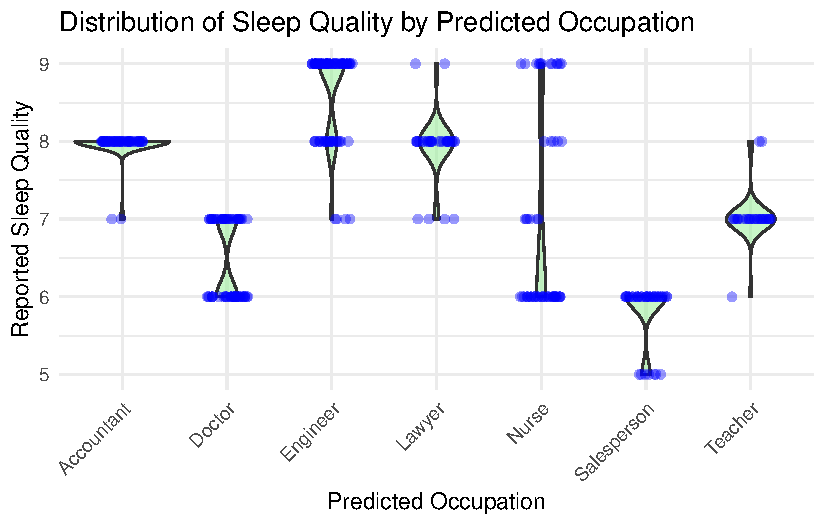
\includegraphics[keepaspectratio]{Final_Project2_files/figure-pdf/unnamed-chunk-7-1.pdf}}

\pandocbounded{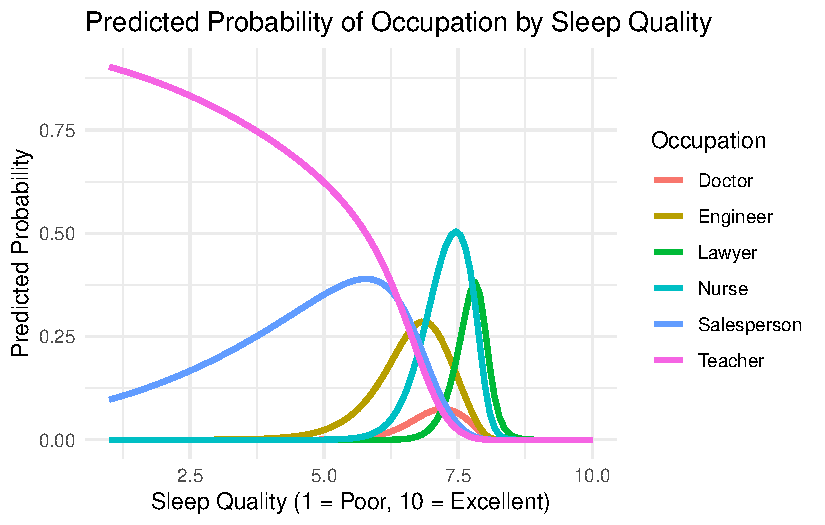
\includegraphics[keepaspectratio]{Final_Project2_files/figure-pdf/unnamed-chunk-8-1.pdf}}

\subsection{Results}\label{results}

In this confirmation set, we will first test how well our exploration
set can be used to predict our confirmation set.

\begin{verbatim}
             Actual
Predicted     Accountant Doctor Engineer Lawyer Nurse Salesperson Teacher
  Accountant          20      0        2      9     0           0       4
  Doctor               0     48        2      4     1           0       3
  Engineer             0      0       24      1    17           0       0
  Lawyer               4      0       10     17     8           0       0
  Nurse                2      2        4      2    22           0       0
  Salesperson          0      0        1      0     4          23       3
  Teacher              0      0        2      0     0           0      18
\end{verbatim}

When running a prediction on this fitted model, we can see that this
model correctly predicts Occupation our key \textbf{X} variable
(Occupation) at a rate above average in some occupations, but shows
extreme accuracy in others such as ``Teacher'', ``Doctor'', and
``Salesperson''. This tells us that this data set may hold some strong
trends within professions, and gives us confidence that our data does
not suffer from high variance.

We used a similar format below to predict quality of sleep, our
\textbf{Y}-variable.

\begin{verbatim}
         Actual
Predicted 1_QoS 2_QoS 3_QoS 4_QoS 5_QoS 6_QoS 7_QoS 8_QoS 9_QoS 10_QoS
   1_QoS      0     0     0     0     0     0     0     0     0      0
   2_QoS      0     0     0     0     0     0     0     0     0      0
   3_QoS      0     0     0     0     0     0     0     0     0      0
   4_QoS      0     0     0     0     0     0     0     0     0      0
   5_QoS      0     0     0     0     4     3     0     0     0      0
   6_QoS      0     0     0     0     0    67     0     0     0      0
   7_QoS      0     0     0     0     1     2    45     0     0      0
   8_QoS      0     0     0     0     0     0     7    72     0      0
   9_QoS      0     0     0     0     0     0     2     3    50      0
   10_QoS     0     0     0     0     0     0     0     0     0      0
\end{verbatim}

We can see similarly here, that Quality of Sleep (QoS) also has strong
predictability. This is a very good sign that our data is significant.

Next, we

\begin{verbatim}
             Df Sum Sq Mean Sq F value Pr(>F)    
Occupation    6  194.8   32.46   41.65 <2e-16 ***
Residuals   356  277.5    0.78                   
---
Signif. codes:  0 '***' 0.001 '**' 0.01 '*' 0.05 '.' 0.1 ' ' 1
\end{verbatim}

\begin{verbatim}
  Tukey multiple comparisons of means
    95% family-wise confidence level

Fit: aov(formula = Quality.of.Sleep ~ Occupation, data = dat)

$Occupation
                               diff         lwr          upr     p adj
Doctor-Accountant      -1.244004568 -1.77482611 -0.713183023 0.0000000
Engineer-Accountant     0.520806521 -0.02143849  1.063051530 0.0690249
Lawyer-Accountant       0.001725129 -0.57365724  0.577107501 1.0000000
Nurse-Accountant       -0.522028878 -1.05035338  0.006295622 0.0552002
Salesperson-Accountant -1.891891892 -2.52388944 -1.259894342 0.0000000
Teacher-Accountant     -0.916891892 -1.51403882 -0.319744960 0.0001469
Engineer-Doctor         1.764811089  1.31168439  2.217937786 0.0000000
Lawyer-Doctor           1.245729697  0.75342996  1.738029431 0.0000000
Nurse-Doctor            0.721975690  0.28560322  1.158348158 0.0000291
Salesperson-Doctor     -0.647887324 -1.20530553 -0.090469118 0.0112477
Teacher-Doctor          0.327112676 -0.19045723  0.844682586 0.4989307
Lawyer-Engineer        -0.519081391 -1.02367743 -0.014485350 0.0391550
Nurse-Engineer         -1.042835399 -1.49303432 -0.592636478 0.0000000
Salesperson-Engineer   -2.412698413 -2.98100572 -1.844391107 0.0000000
Teacher-Engineer       -1.437698413 -1.96697787 -0.908418951 0.0000000
Nurse-Lawyer           -0.523754008 -1.01336027 -0.034147745 0.0272005
Salesperson-Lawyer     -1.893617021 -2.49362404 -1.293610007 0.0000000
Teacher-Lawyer         -0.918617021 -1.48179725 -0.355436790 0.0000403
Salesperson-Nurse      -1.369863014 -1.92490384 -0.814822185 0.0000000
Teacher-Nurse          -0.394863014 -0.90987163  0.120145604 0.2598364
Teacher-Salesperson     0.975000000  0.35409099  1.595909012 0.0000925
\end{verbatim}

\begin{verbatim}
[1] NA
\end{verbatim}

Evaluate accuracy or confusion matrix table(Predicted =
confirmation\_set\(Predicted, Actual = confirmation_set\)Occupation)

\subsection{Discussion}\label{discussion}

\section{}\label{section}

\section{}\label{section-1}

\section{}\label{section-2}

\section{}\label{section-3}

\subsection{Final Report}\label{final-report}

Your final report should document your analysis, communicating your
findings in a way that is technically precise, clear, and persuasive.

Page limits:

\begin{itemize}
\tightlist
\item
  Main report: 4 pages
\item
  Appendix: 1 additional page
\end{itemize}

You must meet these page limits using standard \texttt{pdf\_document}
output in a \texttt{.Rmd} file, or in a
\texttt{documentclass:\ scrartcl} in a \texttt{.qmd} file. (This
assignment prompt has been generated as a \texttt{scrartcl}).

The one-page appendix is intended for extra information that will help
your instructor assess your model building process. Please include the
following elements:

\begin{enumerate}
\def\labelenumi{\arabic{enumi}.}
\tightlist
\item
  \textbf{A Link to your Data Source.} If you used specialized code to
  access your data, please include that here. Please make sure your
  instructor has the ability to access the data.
\item
  \textbf{A List of Model Specifications you Tried.} We are interested
  in seeing how you arrived at your final model. In just a sentence,
  please provide a reason or something that you learned from each
  specification.
\item
  \textbf{A Residuals-vs-Fitted-values Plot.} Please generate this plot
  for your final model that includes variable transformations. Your
  instructor will use this plot to assess how well you have captured the
  shape of the relationship between your X and your Y variable. For
  example, if there is a clear parabolic pattern in your
  residuals-vs-fitted plot, that is a signal that you should have
  included a square term.
\end{enumerate}

\subsection{Evaluation Criteria}\label{evaluation-criteria}

We present the following criteria to guide you to a professional-quality
report. Moreover, these criteria are also the ones we will use to grade
your report. The descriptions below are copied directly from our grading
rubric.

\subsubsection{1. Intro}\label{intro}

An introduction that is scored in the top level has very successfully
made the case for the study. It will have explained why the topic is
interesting, and provided compelling reasons to care about not just the
general area, but rather about every concept in the research question
and the statistical results to be generated. The introduction will be
engaging from the very first sentence, and create a logical story that
leads the reader step-by-step to the research question. After reading
the introduction, no part of the research question will appear arbitrary
or unexpected, instead flowing naturally from the background provided.

\subsubsection{2. Description of the Data
Source}\label{description-of-the-data-source}

A report that is scored in the top level will describe the provenance of
the data; the audience will know the source of the data, the method used
to collect the data, the units of observation of the data, and important
features of the data that are useful for judging the analysis.

\subsubsection{3. Data Wrangling}\label{data-wrangling}

A report that is scored in the top level on data wrangling will have
succeeded to produce a modern, legible data pipeline from raw data to
data for analysis. Because there are many pieces of data that are being
marshaled, the reports that score in the top level will have refactored
different steps in the data handling into separate files, functions, or
other units. It should be clear what, and how, any additional features
are derived from this data. The analysis avoid defining additional data
frames when a single source of truth data would suffice.

\subsubsection{4. Operationalization}\label{operationalization}

A report that is scored in the top level on operationalization will have
precisely articulated and justified the decisions leading to the
variables used in the analysis. The reader will be left with a clear
understanding of the concepts in the research question, and how they
relate to the operational definitions, including any major gaps that may
impact the interpretation of results. You should also list how many
observations you remove and for what reasons. When there is more than
one reasonable way to operationalize a concept, the report will explain
the alternatives and provide reasons for the one that was selected. Note
that there is often more than one way to operationalize a concept; we
are less interested in whether you make the best possible choice, and
more in how well you defend your decisions.

\subsubsection{5. One or More Data
Visualization(s)}\label{one-or-more-data-visualizations}

This is a task of description, and one of the most effective ways to
describe relationships between variables is through visualization.

You are required to include at least one plot in your main report that
highlights the relationship between your \(Y\) and your \(X\) variables
In your text, you should provide your interpretation of what this plot
means, and link to the plot. For example, we might write that
Figure~\ref{fig-dist} displays 300 observations from a synthetic model
of Earnings and Age, showing an increasing trend though the relationship
is less positive for higher ages.

Include a visual representation of your final model predictions on the
plot. A report that is scored in the top level will have plots that
effectively transmit information, engage the reader's interest, maximize
usability, and follow best practices of data visualization. Titles and
labels will be informative and written in plain English, avoiding
variable names or other artifacts of R code. Plots will have a good
ratio of information to space or information to ink; a large or
complicated plot will not be used when simple plot or table would show
the same information more directly. Axis limits will be chosen to
minimize visual distortion and avoid misleading the viewer. Plots will
be free of visual artifacts created by binning. Colors and line types
will be chosen to reinforce the meanings of variable levels and with
thought given to accessibility for the visually-impaired. Your report
will be free of ``output dumps'' - code output that has not been
formatted for human-readability. Every single plot and table in the
report will be discussed in the narrative of the report.

\begin{figure}[t]

\centering{

\pandocbounded{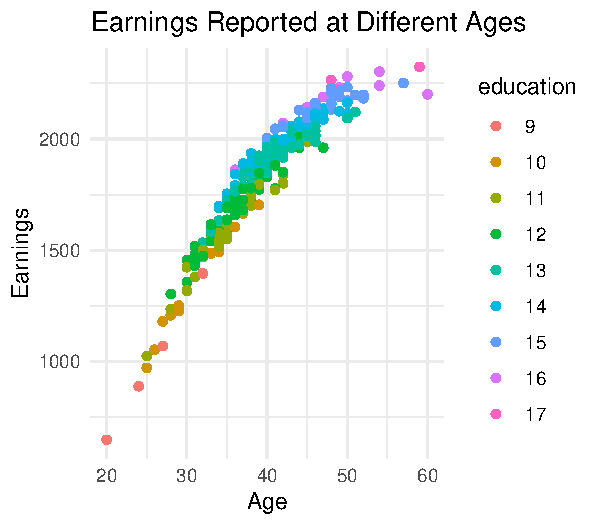
\includegraphics[keepaspectratio]{Final_Project2_files/figure-pdf/fig-dist-1.pdf}}

}

\caption{\label{fig-dist}Synthetic data showing a hypothetical
relationship between Earnings, Age, and Education. An increasing trend
can be seen with decreasing slope for higher ages.}

\end{figure}%

\subsubsection{6. Model Specification}\label{model-specification}

A report that is scored in the top level will have chosen a set of
regression models that strongly support the goal of the study. Variables
transformations will be chosen to inform the reader of the shape of the
joint distribution, and will be human-understandable. A reason will be
provided for the chosen variable transformations. Ordinal variables will
not be treated as metric. All model specifications will be displayed in
a regression table, using a package like
\href{https://cran.r-project.org/web/packages/stargazer/vignettes/stargazer.pdf}{\texttt{stargazer}}
to format your output. Displayed standard errors will be correctly
chosen.

\#```\{r report models, message = FALSE, warning = FALSE, results =
`asis'\} \#\#\textbar{} results: asis \#\#\textbar{} warning: FALSE
\#\#\textbar{} message: FALSE \#\#\textbar{} tbl-cap: Regression
Results. \#\#\textbar{} \#\textbar{} tbl-pos: t \#stargazer( \#
model\_one, \# model\_two, \# model\_three, \# header = FALSE, \# se =
list( \#\# sqrt(diag(vcovHC(model\_one))), \#
sqrt(diag(vcovHC(model\_two))), \# sqrt(diag(vcovHC(model\_three))) \#
), \# type = ifelse(knitr::is\_latex\_output(), ``latex'', ``html''), \#
covariate.labels = c(``Age'', ``\(\\text{Age}^2\)'', ``Education'',
``Intercept''), \# digits = 2, \# omit.stat = c(`ser', `f'), \#
star.cutoffs = c(0.05, 0.01, 0.001) \#)

```

\subsubsection{7. Model Assumptions}\label{model-assumptions}

A report that scores in the top-level has provided an thorough and
precise assessment of the assumptions supporting the regression. The
list of assumptions is appropriate given the sample size and modeling
goals. Each assumption is evaluated fairly, and discussed defensively -
without overstating how credible the assumption is or rendering a final
up-or-down judgement on the assumption. The report will not miss any
important violations of any assumption. Where possible, the report
discusses the consequences for the analysis of a violated assumption.

\subsubsection{8. Model Results and
Interpretation}\label{model-results-and-interpretation}

A report that scores in the top level will correctly interpret
statistical significance, clearly interpret practical significance, and
comment on the broader implications of the results. It may want to
include statistical tests besides the standard t-tests for regression
coefficients. When discussing practical significance, comment on both
the direction and magnitude of your coefficients, placing them in
context so the reader can understand if they are important. To help the
reader understand your fitted model, you may want to describe
hypothetical datapoints (e.g.~a hypothetical person with 1 cat is
predicted to spend \$2400 on pet care. That rises to \$3200 for a
hypothetical person with 2 cats\ldots).

\subsubsection{9. Overall Effect}\label{overall-effect}

A report that scores in the top level will have met expectations for
professionalism in data-based writing, reasoning and argument for this
point in the course. It can be presented, as is, to another student in
the course, and that student could read, interpret and take away the
aims, intents, and conclusions of the report.

\section{References}\label{references}

\phantomsection\label{refs}
\begin{CSLReferences}{0}{1}
\end{CSLReferences}




\end{document}
